\subsubsection{\texttt{RF-6}: gestión de matriculación de usuarios en cursos}
\label{subsec:rf6}

Cuando utilizan la extensión para Visual Studio Code, los docentes tienen la posibilidad de inscribir y eliminar estudiantes y otros profesores de sus cursos. Equivalentemente, se añade a la aplicación web la posibilidad de gestionar las matrículas de un curso. Para ello, tal como introduce el requisito \referenciaConTT{subsec:rf1}{RF-1.2}, los docentes disponen de un botón ``Manage enrolled users'' (gestionar usuarios inscritos) que despliega una ventana modal.

Este modal, tal como se muestra en la \referenciaFigura{fig:reqf6-1}, muestra una lista con todos los usuarios inscritos en el curso, diferenciando a los profesores de los estudiantes. A excepción del profesor creador, cada uno de estos usuarios puede ser eliminado del curso haciendo uso del botón dispuesto en cada fila. Adicionalmente, en la parte inferior se muestra un desplegable que contiene todos los usuarios potencialmente matriculables; esto es, a todos los usuarios salvo a aquellos que ya están matriculados. El profesor puede escoger uno de ellos y, mediante el botón adyacente, inscribirlo en el curso.

\begin{figure}[ht]
    \centering
    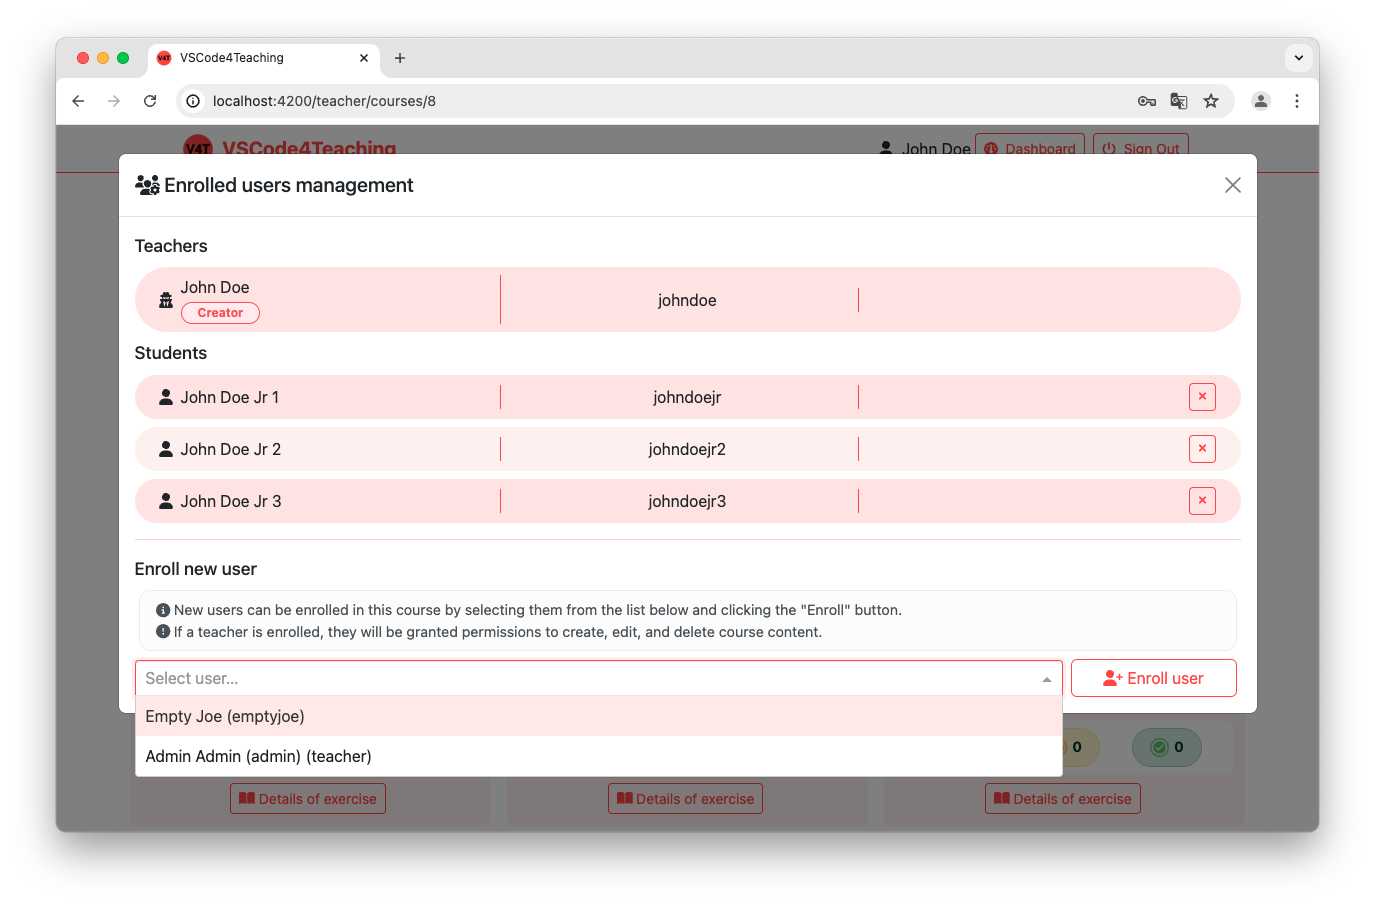
\includegraphics[width=\textwidth]{imagenes/utilizadas/4-3-implementacion/rf6-1.png}
    \caption{Visualización de la lista de usuarios inscritos a un curso y de las capacidades para añadir nuevos usuarios o revocar inscripciones.}
    \label{fig:reqf6-1}
\end{figure}
